\documentclass{article}
\usepackage[english]{babel}
\usepackage[a4paper,top=2cm,bottom=2cm,left=3cm,right=3cm,marginparwidth=1.75cm]{geometry}

% Useful packages
\usepackage{authblk}
\usepackage{amsmath}
\usepackage{graphicx}
\usepackage[colorlinks=true, allcolors=blue]{hyperref}

\begin{document}
\title{Applications of LLMs - interactive communication system}
\author{Oliver Dassinger}
\setlength{\affilsep}{0em}
\affil{\textit{Friedrich Alexander University}}
\affil{\textit{Pattern Recognition Lab}}
\affil{\textit{oliver.dassinger@fau.de}}

\date{}

\maketitle

\begin{abstract}
\noindent The recent advancements in Large Language Models (LLMs) have significantly improved capabilities in various domains, such as content creation, translation, code generation, customer support, and education. These improvements allowed the creation of sophisticated interactive applications like chatbots. Despite this progress, they still face limitations as their training relies on large static datasets which quickly become outdated as well as the inability to access private data. This project develops a document-based question-answering chatbot using the LangChain framework to utilize the OpenAI API for deploying an LLM. It makes use of the Retrieval-Augmented Generation (RAG) technique to dynamically generate questions based on the document embeddings stored through ChromaDB. By reversing the typical question-answer interaction format, the system proactively questions the user about the content of the provided document. The user response is then evaluated by using the cosine similarity to determine the accuracy against the correct, model-generated answer. This approach successfully demonstrates the advantages of using RAG for interactive question-answering, significantly enhancing the adaptability and interactivity of chatbots. 
\end{abstract}
\begin{quote}
\textbf{KEYWORDS:}\\
Interactive question answering, Large Language Models (LLMs), Retrieval-Augmented Generation (RAG), Chatbots, Information retrieval
\end{quote}

\section{Introduction}
Large language models, especially in their application as interactive communication systems like chatbots, have experienced a tremendous increase in popularity, becoming indispensable in today's digital landscape. Their rise in popularity has been driven by their ability to generate human-like text, making it possible to interact with them in a more natural, intuitive way. This led to a wide range of applications across different domains in different sectors including content creation, customer support, education, and more. However, despite these advancements, the application of LLMs still faces significant limitations and problems to overcome.
\newline
One of the main issues, particularly when using large language models in the domain of chatbots, is their dependence on large, static datasets. This can limit their ability to provide up-to-date information and adapt to new information as they are trained only on data available up to a certain point, thus excluding recent developments and real-time information. Furthermore, LLMs are often limited to information included within their training datasets, thus making it challenging to incorporate confidential or proprietary data directly into their knowledge. These limitations not only diminish the relevance of information provided by chatbots but also reduce their usefulness in real-world applications.
\newline
To address these issues, this project combines a classical large language model with a retrieval-augmented generation approach to build a document-based question-answering chatbot. Utilizing the LangChain framework\footnote{https://www.langchain.com/langchain}, which integrates the capabilities of the \mbox{OpenAI} API\footnote{https://python.langchain.com/docs/integrations/platforms/openai/}, it was possible to incorporate information directly obtained from local documents by combining the extensive global knowledge of the LLM with the local information from the documents. As a result, the system is capable of dynamically generating contextually relevant questions by leveraging the information stored in the document embeddings of the lecture notes. These embeddings are created from the provided course transcripts of the pattern recognition lecture held at the Friedrich-Alexander-University Erlangen-Nuremberg\footnote{https://lme.tf.fau.de/category/lecture-notes/lecture-notes-pr/} and are stored in \mbox{ChromaDB}\footnote{https://www.trychroma.com/}, an open-source embedding database. To conclude the chatbot, an evaluation mechanism has been implemented to assess the accuracy of the user's response.

\section{Related work}
Encountering similar problems with LLMs as in this project, such as outdated knowledge and hallucinations, Gao et al. \cite{gao2024retrievalaugmented} conducted a comprehensive analysis of different RAG approaches to enhance LLMs, categorizing their development into three paradigms: the Naive RAG, the Advanced RAG, and the Modular RAG. Each of them improves the integration of the LLM with the knowledge of an external database, aiming to mitigate the limitations of LLMs. While the Naive RAG paradigm encompasses the traditional RAG approach that indexes the documents, retrieves the most relevant ones with respect to the query, and uses their information to generate the augmented output, the authors highlight its significant disadvantages, such as retrieval errors, limited adaptability, or missing crucial information. To mitigate these issues, the Advanced RAG paradigm improves the retrieval process through enhanced indexing and querying, while the Modular RAG paradigm improves the other two RAG paradigms even further by introducing adaptable modules that can be individually fine-tuned to optimize specific components of the RAG system.
\newline
Alan and his team \cite{alan2024ragbased} investigated a RAG-based question-answering system, "MufassirQAS", for religious contexts. Addressing similar issues such as outdated or inaccurate information from static LLMs, they employed a vector database enabling their system to access and retrieve relevant information from Turkish translations and interpretations of Islam. By augmenting the model's knowledgebase with the retrieved information from their dataset and including detailed references such as page numbers and document names, Alan et al. enhanced transparency and accuracy, allowing the user to verify the origin of the information provided. They stated that their system provided similar answers for general questions, but gave more precise and detailed responses to non-trivial queries.
\newline
Patil et al. \cite{patil2023gorilla} investigated the integration of LLMs with the ability to interact with external data via API calls. Their proposed model, "Gorilla", a fine-tuned large language model combined with a document retriever, significantly outperformed other LLMs like GPT-4 and overcame the inability to generate accurate API calls. By using a retrieval system that adapts to changes in API documentation, Gorilla ensures accuracy even as APIs are updated without the need for constant retraining. Evaluating the model's capabilities on the APIBench dataset, a dataset consisting of a large corpus of API calls, they showed that Gorilla outperformed state-of-the-art LLMs like GPT-4 by over 20\% in accuracy while at the same time reducing hallucinations. This approach emphasizes the advantages of combining an LLM with a retrieval-augmented approach to enhance the accuracy and responsiveness of the system.

\section{Methodology}
This section describes the frameworks and technologies used to develop the interactive examination chatbot. It explains how the LangChain framework was leveraged to combine the OpenAI API with a retrieval-augmented generation system, enabling access to both the large language model and the embedding model. This architecture made it possible to utilize the power of OpenAI's LLM and enhanced it even further by incorporating contextual data retrieved from ChromaDB, the local vector database used in this project. To ensure these components are accessible through a user-friendly interface, Streamlit\footnote{https://streamlit.io/} was used to create the interactive web application, completing the setup of the system.
\subsection{Retrieval-Augmented Generation (RAG)}
Large language models are powerful models that can generate human-like text, yet they face limitations due to their reliance on static training datasets, which can lead to false, outdated, or generic information. Retrieval-augmented generation addresses these issues by integrating real-time, retrieved information from a database into the response generation process. RAG works by making use of a vector database where document embeddings are stored. These embeddings contain the semantic information of the documents as numerical vectors. When a query is made, it is transformed into an embedding using the same model that was used to create the document embeddings. The query embedding is then compared with the document embeddings stored in the database to retrieve the most relevant document. This retrieval is based on similarity search algorithms like the cosine similarity or nearest neighbor search. The most relevant embeddings are then fed to the LLM, augmenting its global knowledge with context-specific information. This allows the system to access relevant information from external knowledge sources, thereby generating more accurate and relevant responses.
\newline
In this project, the goal was to build an interactive chatbot that is able to generate questions and corresponding answers based on the provided document. To achieve this, I implemented the RAG approach, which directly utilizes the content of the documents as context for the language model. This enables the system to generate relevant questions and answers that are contextually dependent on the provided documents.
\subsection{System Architecture}
As the goal was to build an interactive communication system that acts as an examination bot, the classical RAG architecture had to be slightly adjusted to fit the project's needs. The resulting architecture is shown in Figure 1. The system's workflow begins when the user uploads a .docx file through the user interface, which is created with Streamlit. This document gets automatically segmented into chunks, each of which is then transformed into embeddings. Each embedding contains the semantic information of the corresponding text chunk, represented as a numerical vector. If the embeddings for the current file don't exist, they are stored in the local vector database. Once these are created and stored, the system uses the vector store retriever to provide the context for the question-and-answer generation by leveraging the embeddings to retrieve the relevant information from the uploaded document. The language model then generates the question and the corresponding answer based on the retrieved context and a predefined template for the question and one for the answer. After the question is displayed in the user interface, the user submits his answer, which, along with the answer generated by the LLM, is evaluated by using a cosine similarity-based grading system. 
\begin{figure}[h]
    \centering
    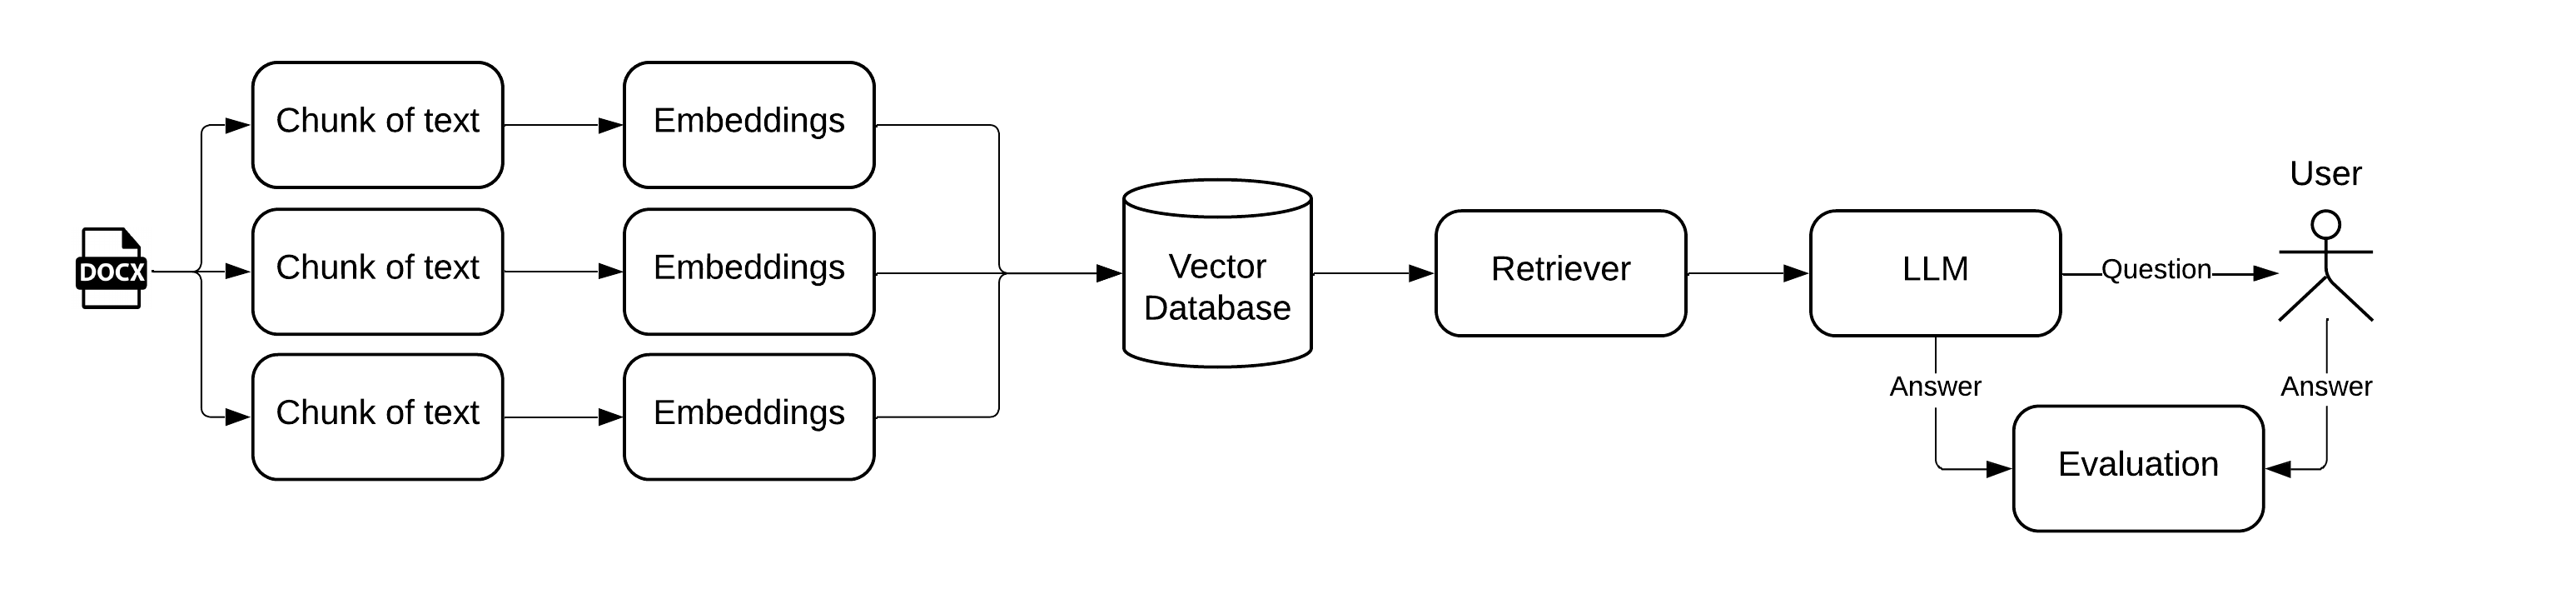
\includegraphics[width=\textwidth]{Images/overview_system_architecture.png}
    \caption{Architecture of the RAG Chatbot}
\end{figure}
\subsection{Dataset}
The dataset for this project, consisting of 43 Word documents, was provided by the project supervisor from the Chair of Pattern Recognition\footnote{https://lme.tf.fau.de/} at the Friedrich-Alexander-University Erlangen-Nuremberg. These documents are transcripts from the pattern recognition lecture series, each covering a specific topic within the field, providing a profound understanding of the key concepts and techniques. Based on the RAG approach utilized in this project, these documents were used as provided without undergoing any preprocessing steps. This straightforward utilization exploits the natural structure and content of the documents, aligning with the core principles of RAG to directly augment the large language model by providing detailed, lecture-specific information from the given materials.
\newline
The documents serve as the basis for creating the embeddings that enable dynamic retrieval of information to generate the questions and corresponding answers, as described in the System Architecture section. Such direct utilization aligns with the project's aim of creating an interactive communication system that functions as an examination bot by using real-time information retrieval.
\subsection{LangChain}
LangChain is a key component in the architecture of the interactive exam chatbot and serves as the integration framework to link the OpenAI API with the retrieval-augmented generation system, thus enabling efficient communication between the large language model, the retriever, and the vector database. It manages efficient workflow throughout the different components of the system, ensuring that the interaction between the LLM, accessed through LangChain's OpenAI API integration, and the vector database is seamless. This integration is crucial to fully utilize the capabilities of the OpenAI's LLM, which relies on meaningful information from ChromaDB to generate contextually relevant questions and answers in an interactive manner.
\subsection{ChromaDB}
ChromaDB is an open-source vector database that is used for storing and managing the embeddings within the interactive chatbot system. It enables including local information stored in the database through efficient storage and retrieval of the created embeddings. While ChromaDB is configured by default to store data ephemerally, it has been set up to persistently store the embeddings locally. This allows the system to quickly access relevant context required for the question-and-answer generation without the need to repeatedly process the same documents. By utilizing ChromaDB's capabilities in this project, I was able to store the created embeddings from the text chunks of the .docx files, enabling real-time data retrieval. After the embeddings are stored, the system leverages ChromaDB to fetch the most relevant embeddings that correspond to the text segments of the document. This is achieved by initializing a retriever that uses cosine similarity to identify the top two most relevant text chunks from the document. By utilizing ChromaDB's capabilities, the system is able to efficiently manage large amounts of documents and ensures quick retrieval of relevant information, thereby enhancing the performance of the chatbot.
\subsection{Streamlit}
Streamlit is an open-source framework specifically developed for creating interactive web applications in data science and machine learning projects. Due to its ease of use and efficient creation of web applications, it was chosen as the primary framework for developing the user interface of the chatbot. Streamlit executes the entire script from start to finish with every user interaction, ensuring that the latest user input is always taken into account. However, this approach implies that the application is stateless by default, resulting in resetting and executing the entire code again with each user interaction. To avoid the reset and maintain state across user interactions, session variables are used. 
\newline
By integrating Streamlit with the backend processes powered by the frameworks mentioned in the previous subsections, I was able to create a fully functional communication system. Users can seamlessly upload a document which is then processed by the system. Questions are displayed in the interface, and the user can reply with the answer in a chat-like format, allowing direct interaction with the system in real-time. 

\section{Implementation}
The implementation of the interactive chatbot is realized through several Python modules, each responsible for a specific functionality within the chatbot. The \textit{main.py} file is the core of the system and the entry point for the Streamlit application. This script manages the integration of the other modules, thereby managing the workflow of the application.
\newline
Upon initiation, the application is activated by initializing the large language model and the embedding model using the OpenAI API key extracted from the environment variables. For the chat functionality, the "gpt-3.5-turbo" model is employed, whereas the "text-embedding-3-large" model is utilized for the embedding processes. These models were chosen due to their cutting-edge capabilities, representing the latest and most advanced models from OpenAI at the time of this project's development. Additionally, session state variables are set up to enable data persistence across user interactions and page refreshes within a session, enhancing the user experience by maintaining state consistency.
\newline
When the user tries to upload a .docx file through the file uploader in the interface, the system checks whether the document and the ChromaDB collection already exists. If not, it is stored in a specific directory, and a corresponding collection is created, where the collection name is inferred based on the file name. This collection serves as the storage container for the embeddings of the document, allowing for efficient storage and retrieval.
\newline
The document then undergoes a preprocessing step where it is segmented into manageable chunks of 2800 tokens, each with a 280-token overlap to ensure contextual continuity. This segmentation is critical given the 16,385 token context window limitation of the "gpt-3.5-turbo" model used in this project. Dividing the text into smaller sections while including a certain overlap ensures that no important information is cut off due to the capacity limits of the model when encountering longer documents. Subsequently, the embeddings for the current file are generated by using OpenAI's "text-embedding-3-large" model and are stored in a designated collection in the database.
\newline
The user interface offers file interaction buttons such as "Chat", "Clear Chat", and "Delete". These buttons become activated as soon as the file is fully processed and removed from the upload form, allowing the user to engage with the uploaded content interactively. 
\newline
After clearing the file uploader, selecting the desired file in the dropdown, and clicking the chat button, the conversation is initiated by creating a retriever for the current collection. This retriever extracts relevant context from the document's embeddings, which, along with a list of previously asked questions, is passed to the LLM. The LLM, guided by a predefined question template, generates a unique question based on the obtained context from the retriever. The template is used to specify the desired output of the language model by instructing it to act as an examination bot and making sure that the questions are unique by including a list of already asked questions in the prompt. Similarly, the LLM generates an answer for the posed question based on the provided content.
\newline
Both the generated question and the answer are then stored in session variables to maintain a record of the dialogue history and previously asked questions. When the user tries to answer the proposed question, the answer is evaluated by comparing the semantic similarity with the model-generated answer. Therefore, the system's answer and the user's answer are embedded with the same embedding model applied to the documents. The cosine similarity between the system's answer and the user's answer is then calculated and depending on the cosine similarity score, the user's response is rated, providing feedback on the accuracy and relevance of the user's answer.
\newline
Below is a screenshot of the chatbot interface, illustrating how the user can interact with the system and the type of questions and responses the chatbot generates based on the uploaded document.
\begin{figure}[h]
    \centering
    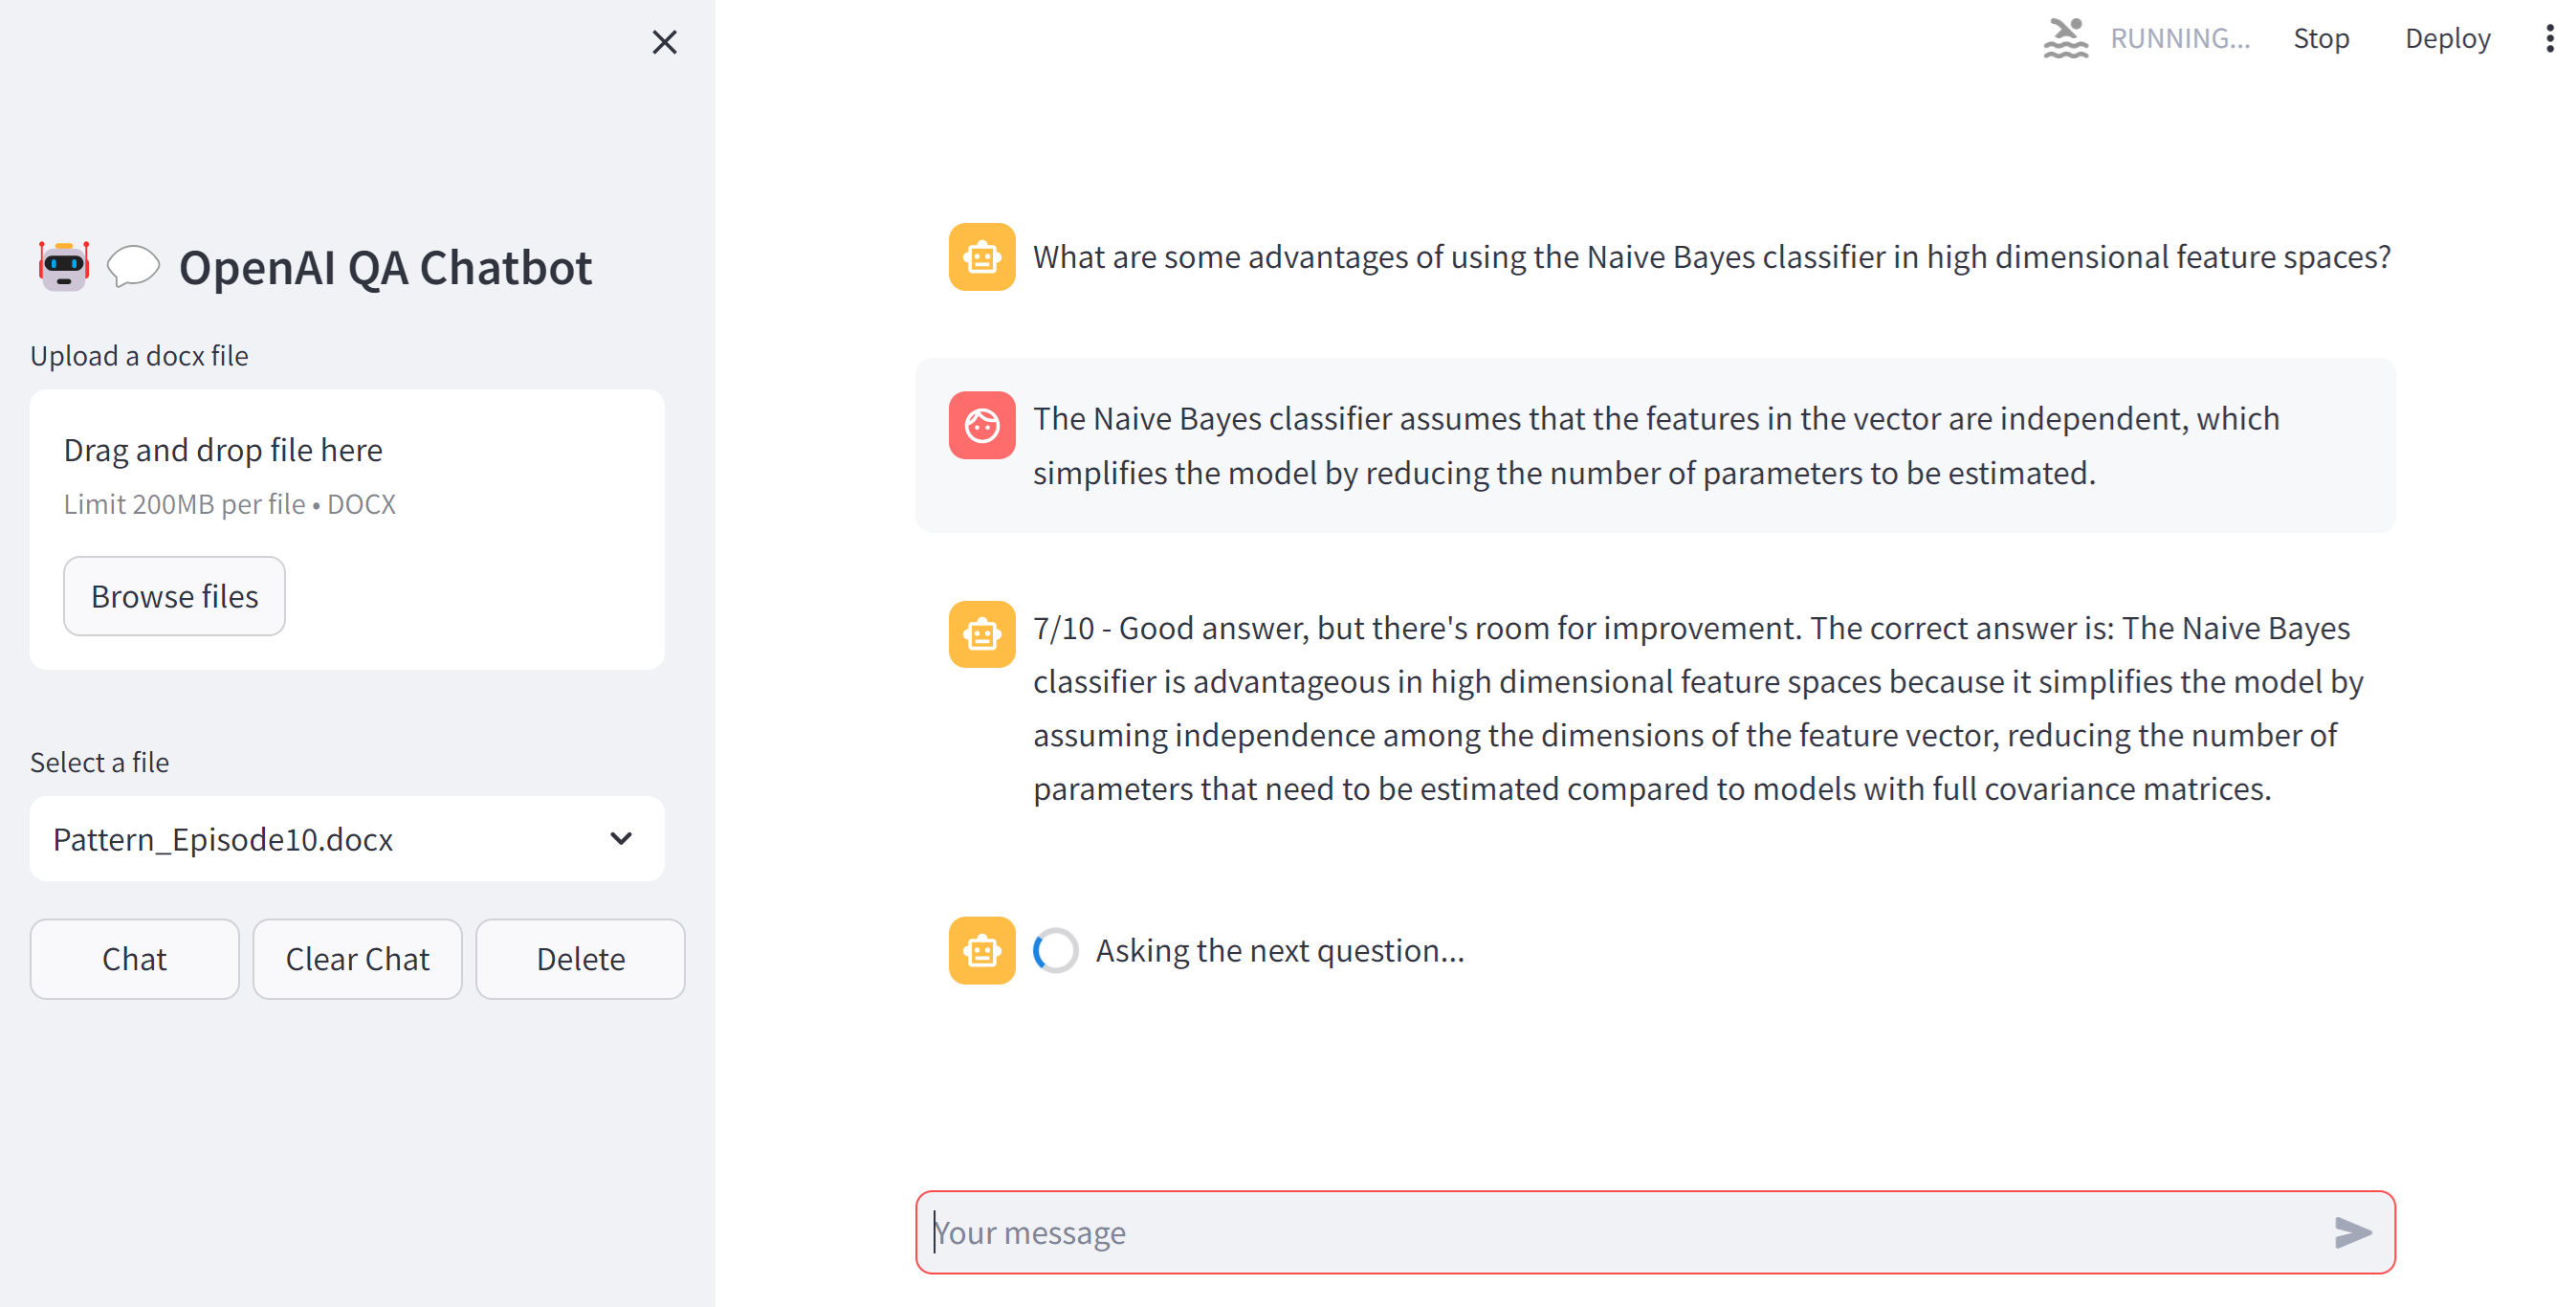
\includegraphics[width=\textwidth]{Images/chatbot_interface.png}
    \caption{User Interface of the QA Chatbot}
\end{figure}

\section{Results And Discussion}
The development of the interactive communication system resulted in a functional chatbot that is able to generate questions and answers based on the retrieved content of the uploaded documents. By utilizing state-of-the-art models from OpenAI, namely "gpt-3.5-turbo" and "text-embedding-3-large", the chatbot demonstrated robust question-answering capabilities. In particular, the application processed the given .docx files of the pattern recognition lecture, segmenting them effectively into manageable chunks without losing contextual information.
\newline
The augmented large language model demonstrates its strength by generating contextually relevant questions derived from the retrieved document segments. This capability not only enhances the chatbot's adaptability, as it dynamically adjusts its focus and complexity of the questions based on the content of the documents but also its relevance, ensuring that the examination topics are precisely tailored to the user's educational needs.
\newline
The resulting chatbot successfully fulfills the initial project's objective of creating an interactive communication system designed to function as an examination bot. Despite meeting the expected outcome, several challenges were encountered. One challenge was to tune the LLM to ask questions in the desired structure through prompt engineering. From time to time, the LLM generated multiple questions within a single query or failed to format the questions and the answers consistently. Additionally, while the OpenAI API offers powerful, state-of-the-art models with stunning capabilities at low cost, its usage is not free. Although manageable, this could be taken into account for future projects, especially when considering scalability and cost-efficiency for larger projects. Exploring alternative solutions, such as utilizing open-source models from platforms like Hugging Face, could offer similar functionalities while reducing costs.

\section{Conclusion}
This project has successfully demonstrated the Retrieval-Augmented Generation (RAG) approach in combination with a Large Language Model (LLM) to build an interactive communication system. By deploying state-of-the-art models from OpenAI within the framework provided by LangChain, the developed Streamlit chatbot not only addresses the static nature of traditional LLM applications but also leverages information from document embeddings stored in a local database to create a dynamic, examination chatbot. The chatbot's ability to generate questions and answers based on the content of the uploaded documents significantly enhances the application's relevance for educational purposes, as it allows to dynamically change the .docx files, resulting in a shift in the topics of the questions generated. This adaptability is crucial for educational purposes where the content can vary widely, ensuring that the chatbot remains responsive and aligned with the specific subjects of the documents.
\newline
Despite the overall success of the application, there were also challenges to overcome. In particular, obtaining the desired output structure for the LLM and considering the economic aspects of using models from OpenAI for larger projects were challenges faced during this assignment. These challenges are crucial for future tasks and highlight the potential benefits of using sustainable open-source solutions, especially for larger projects.
\newline
This prototype highlights how AI can be used in an educational context, enhancing the learning experience by probing users with contextually relevant questions and evaluating their responses to provide insightful feedback. It lays the foundation for further research and development of AI-driven educational tools, showcasing the potential of how AI can be used to transform educational processes, making them more engaging, responsive, and customizable to meet the individual needs of the users.

\section{References}

\bibliographystyle{apalike}
\bibliography{references}

\end{document}